\documentclass[a4paper, 11pt, oneside, article]{memoir}
\newsubfloat{figure}
\linespread{1.25}

\usepackage{minted} 
\usepackage[T1]{fontenc} 
\usemintedstyle{algol}
\usepackage[]{microtype}
\usepackage[]{siunitx} 
\usepackage[]{eulervm}
\usepackage[]{booktabs} 
\usepackage[]{palatino} 
\usepackage[]{amsmath, amssymb} 
\usepackage[]{graphicx} 
\usepackage[]{svg} 
\usepackage[]{bm} 
\usepackage[]{commath} 
\usepackage[]{geometry} 
\newcommand*{\github}[1]{\def\@github{\color{gray!70}#1}}
\newcommand{\githublogo}{\raisebox{-1pt}{\includegraphics[height=9pt]{imgs/github}}}
\usepackage[backend=biber]{biblatex} 
\addbibresource{../../FYS-STK4155.bib}

\usepackage[]{hyperref} 
\usepackage[noabbrev, capitalize]{cleveref} 

\setlength{\parskip}{1em}
\setlength{\parindent}{0pt}

\newcommand{\OLS}{\mathrm{OLS}}
\newcommand{\Ridge}{\mathrm{ridge}}
\newcommand{\Lasso}{\mathrm{lasso}}
\newcommand{\X}{\bm{X}}
\newcommand{\y}{\bm{y}}
\newcommand{\yhat}{\hat{\bm{y}}}
\newcommand{\transpose}[1]{#1^{\top}}
\newcommand{\mat}[1]{\bm{#1}}
\newcommand{\cost}{\mathcal{C}}

\title{\textsc{Regression and Classification using Feed Forward Neural Networks}}
\author{Ivar Stangeby}
\begin{document}
	\maketitle
	
	 \begin{abstract}
		 In this project we compare the performance of dense neural
		 network architectures to more classical methods of linear and
		 logistic regression in the context of fault detection of
		 credit card loans and linear regression of the franke function.
		
		 Our results indicate that for classification tasks, neural
		 nets has a slight edge over non-regularized logistic
		 regression, with the regularized methods falling behind. For
		 regression, again the non-regularized methods come out on top,
		 with the neural net and the ordinary least squares methods
		 winning by a long shot.


	 The numerical experiments are performed using \textsc{Python} with the
	 \texttt{scikit-learn} library resonsible for fitting the models,
	 \texttt{PyTorch} for handling data-sets and representing the nerual
	 network architecture, and finally \texttt{skorch} for wrapping the
	 neural networks in a \texttt{scikit-learn} friendly API. All relevant code can
	 be found on GitHub:
	
		  \centering{\href{https://github.com/qTipTip/FYS-STK4155}{\githublogo \, \color{gray!50}\textit{github.com/qTipTip}}}
	  \end{abstract}
	\chapter{Introduction}
	

	In this project we make a comparative study on feed forward neural
	networks in a regression and classification setting. In particular, we
	compare feed forward neural networks in this context with the standard
	methods of ordinary least squares for linear regression, and logistic
	regression for classification. 

	Neural networks are a very flexible framework in a wide range of tasks.
	In this day and age where artificial intelligence is gaining traction,
	it is certainly of interest to see how these methods perform in
	settings where many classical methods have been developed. 

	\chapter{Background}

	\section{Neural Networks}

	\subsection{Construction}
	Neural networks has gained a widespread use in the approximation of
	functional relationships. In it's simplest form, a neural network
	consists of a set of \emph{neurons}, being entities that take as input
	a set number of parameters \( x_1, \ldots, x_n \), and computes a
	linear combination of these (often with added bias):
	\begin{equation}
		z = \sum_{i = 0}^n w_ix_i + b.
	\end{equation}
	The
	neuron then decides on whether to ``fire'' or not, by evaluating a
	so-called scalar activation function, \( a = g(z) \). In the architecture
	discussed herein, namely \emph{fully connected} or \emph{dense} neural
	networks, each neuron takes into account all possible parameters. 
	
	By combining a set number of neurons we obtain what is called a
	\emph{layer}. A neural network typically consists of three types of
	layers: an \emph{input layer}, a set number of \emph{hidden layers},
	and finally an \emph{output layer}. 

	\begin{figure}[htbp]
		\centering
		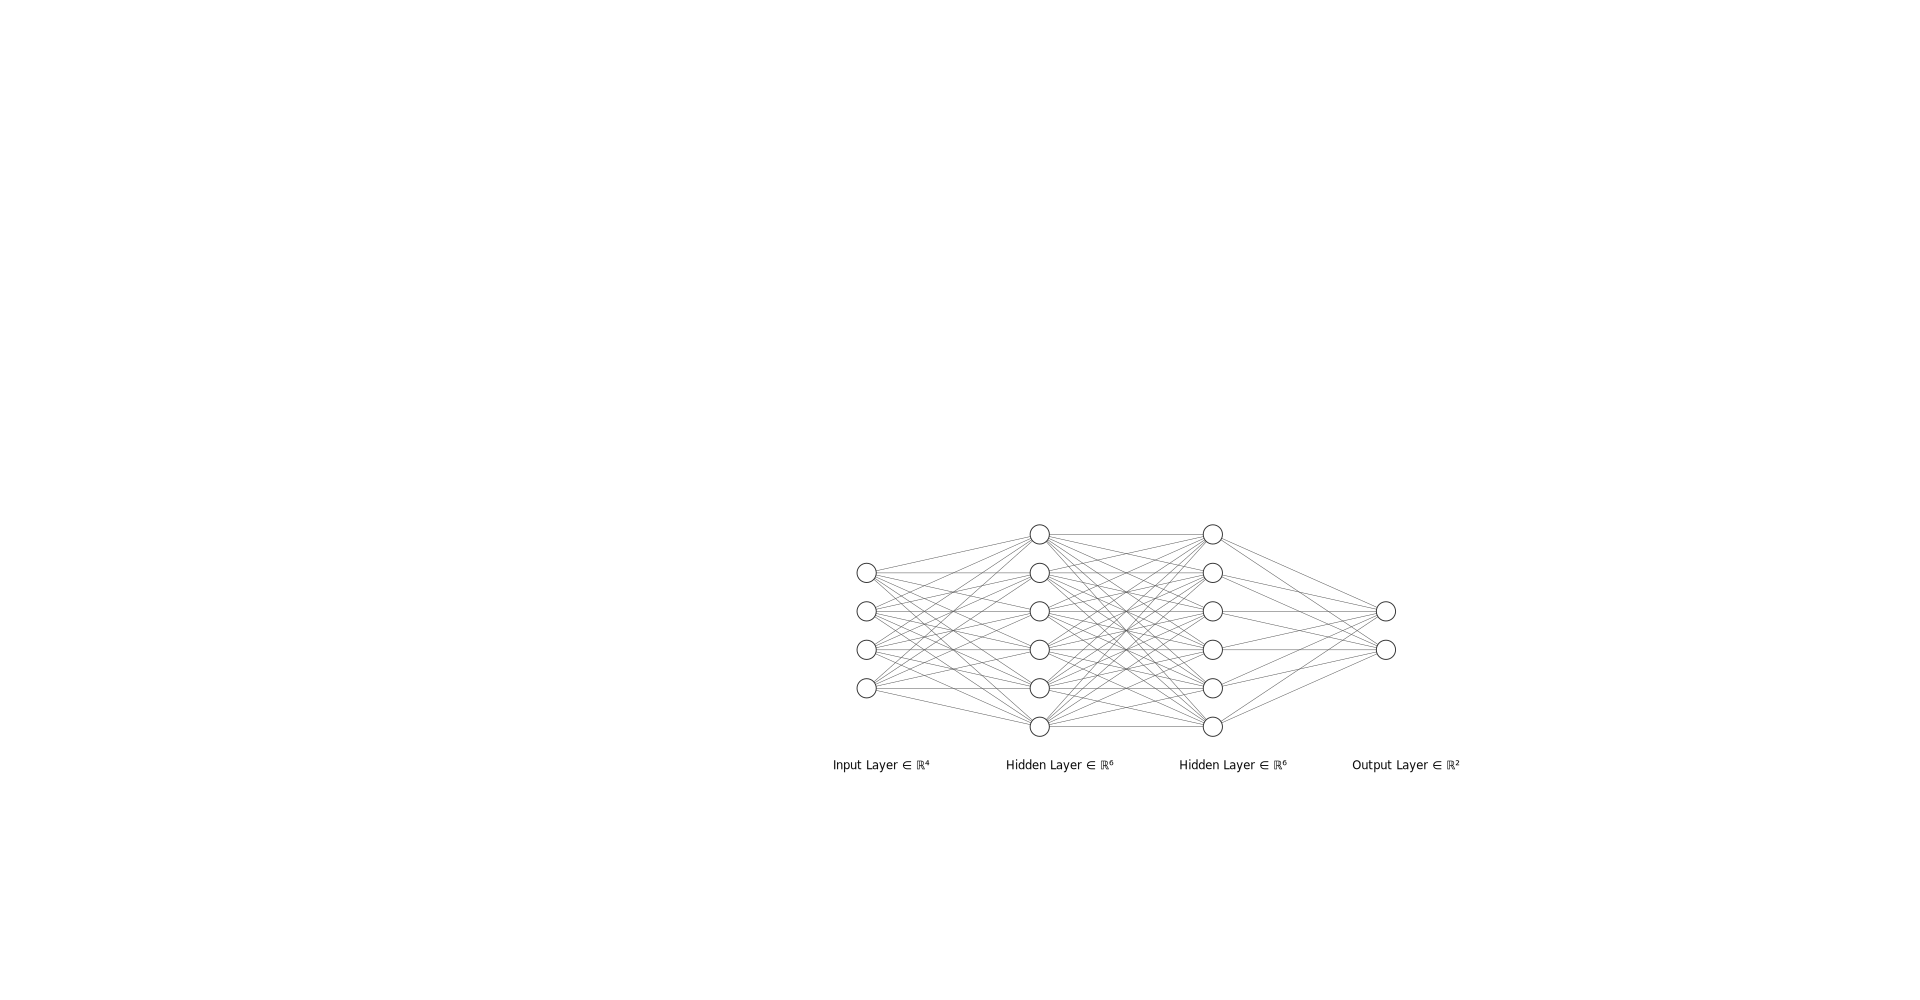
\includegraphics[width=0.8\textwidth]{imgs/fcc_nn.pdf}
		\caption{A simple feed forward neural network. This specific
		network has an input layer of four nodes. Two hidden layers
	consisting of six nodes each, and finally, an output layer of size
two.}%
\label{fig:fc_nn}
	\end{figure}
	
	For a network consisting of \( L \) layers, with each layer having \(
	n^{[\ell]} \) nodes and with activation function \( g\), the
	activations in each layer are given as 
	\begin{equation}
		a^{[\ell]}_k = g\left(\sum_{j = 1}^{n^{[\ell]}} w_{jk}^{[\ell]} a^{[\ell - 1]}_j  + b^{[\ell]}_k \right)
	\end{equation}
	for \( k = 1, \ldots, n^{[\ell]} \) and \( \ell = 1, \ldots, L \). 
	A matrix formulation reads:
	\begin{equation}
	\mat{a}^{[\ell]} = g\left(\mat{W}^{[\ell]} \mat{a}^{[\ell - 1]} + \mat{b}^{[\ell]}\right).
	\end{equation}
	We use the convention that the network input \( \mat{x} = (x_1, \ldots,
	x_{n^{[0]}}) = \mat{a}^{[0]} \) and the network output \( \yhat =
	\mat{a}^{[L]} \).
	
	\subsection{Optimization}
	
	We initialize such a network by specifying the initial weights and
	biases for each layer. That is, the matrices \( \mat{W}^{[\ell]} \) and
	\( \mat{b}^{[\ell]} \) are (most commonly) drawn from some random
	distribution. It is our goal to iteratively optimize these weights and
	biases in order for the network to produce desired output. We therefore
	choose a \emph{cost} function  \( \cost \) which in some way
	incorporates our problem at hand. For example, in regression problems,
	our cost function is typically the mean squared error (MSE) between our
	target-data and our prediction, while in classification, we often use
	cross entropy loss.
	
	We optimize the network by computing the gradient of the cost function
	\( \cost \) with respect to weights and bias' and perform gradient
	descent. That is
	\begin{align}
		\begin{split}
			\mat{W}^{[\ell]} \leftarrow &\mat{W}^{[\ell]} - \lambda \dpd{\cost}{{\mat{W}^{[\ell]}}}, \\ 
			\mat{b}^{[\ell]} \leftarrow &\mat{b}^{[\ell]}\;\, - \lambda \dpd{\cost}{{\mat{b}^{[\ell]}}}
		\end{split}
	\end{align}
	Here \( \lambda > 0 \) is the \emph{learning rate}.

	\subsection{Neural Network Architecture}

	In this paper we study two use-cases of feed forward neural networks,
	namely regression, and classification. The architectures are tailored
	to the data-sets at hand. 
	
	\paragraph{Credit Card Data}

	The credit-card data-set consists of 33 numerical features describing a
	users payment history.  The task at hand is then to predict whether the
	user is prone to defaulting or not. This is therefore a binary
	classification problem. Our network therefore needs to have an input
	layer of size 33, and an output layer of size two (one probability
	value for each class). We---rather arbitrarily---decide on three hidden
	layers of size 20. We use the \emph{rectified linear unit} as our
	activation function for the hidden-layers, and (since we are predicting
	probabilities) we use the \emph{softmax} function as our
	output-activation. These are defined as follows:
	\begin{align}
		\mathrm{RELU}(\mat{x}) &= \max\{\mat{0}, \mat{x}\}, \\
		\mathrm{Softmax}_k(\mat{x}) &= \frac{\exp{x_k}}{\sum_{i=1}^n \exp{x_i}}.
	\end{align}
	Note that the softmax takes as input a vector, and spits out a scalar,
	and that the RELU takes the element-wise maximum.
	Our cost function \( \cost \) is chosen to be \emph{binary cross
	entropy} (or \emph{log-loss}) defined as
	\begin{equation}
		\cost(\mat{y}, \yhat) = -(\mat{y} \log(\yhat) + (1 - \mat{y}) \log(1 - \yhat)).
	\end{equation}

	\paragraph{Regression Data}
		
	For our regression task, we create a synthetic data-set by noisy
	sampling of points from the Franke test-function
	\cite{frankeCriticalComparisonMethods1979}, and our goal is to create a
	neural network that approximates the Franke function. Thus, our network
	should take as input a set of two values, and return a scalar. Again,
	we use a rectified linear unit as our activation function for the
	hidden layers, however, since we want an unrestrained output range, we
	do not add the softmax activation to the final layer, as this would
	squeeze the network output between zero and one.  Our cost function is
	the mean squared error (MSE):
	\begin{equation}
		\cost(\mat{y}, \yhat) = \frac{1}{n} (\y - \yhat)^T (\y - \yhat).
	\end{equation}

	\chapter{Implementation}	
	
	While implementing backpropagation is a great exercise in programming,
	due to time-constraints, we have had to resort to using machine
	learning frameworks in the implementation.

	For defining our neural networks we use the Pytorch-library, and for
	standard methods like linear regression and logistic regression, we
	resort to the scikit-learn toolkit. In addition to this, we use the
	Skorch-library for wrapping the Pytorch modules in a scikit-learn
	compatible API.

	\subsection{Data Wrangling}
	
	We subclass the PyTorch dataset-class for loading the credit card data
	and the sampled Franke data as shown in \cref{lst:datasets}. This
	enables us to write lean training loops as the \texttt{DataLoader}
	class works as a batched iterator.

	\subsection{Neural Network}	
	
	We implement a generic neural network that will suffice for both the
	credit card data (the classification task) and the Franke sampled data
	(the regression task). By subclassing \texttt{torch.nn.Module}, we only
	need to register the different layers, and implement the
	\texttt{forward}-method. The auto-grad framework then takes care of the
	back-propagation of gradients for us. We allow for the user to specify
	the number of input features, the number of output features, the number
	of hidden layers and the the number of hidden units (which we take as
	constant across the hidden layers). Furthermore, we also with to be
	able to specify the final activation function, as this needs to be
	specially tailored (as much else) to the task at hand. The generic
	architecture is layed out in \cref{lst:neural_network}.
	
	\begin{listing}
	\begin{minted}[frame=lines,tabsize=3]{python}
class CreditCardData(torch.nn.utils.data.Dataset):
	def __init__(self, *args, **kwargs):
		super().__init__()
		
		self.X, self.y = self.fetch_data(*args, **kwargs)
		self.num_features, self.num_items = self.X.shape

	def __getitem__(self, index):
		return self.X[index], self.y[index]

	def __len__(self):
		return self.num_items

		super().__init__()	
	def fetch_data(self):
		# Handles the loading and preprocessing of data
		...

class FrankeData(torch.nn.utils.data.Dataset):
	...
	\end{minted}
	\caption{Interfacing the data-sets with a PyTorch API, which facilitates easy iteration as shown in \cref{lst:training_loop}}
	\label{lst:datasets}
	\end{listing}
	
	\begin{listing}
	\begin{minted}[frame=lines,tabsize=3]{python}
credit_card_data = CreditCardData('path_to_dataset')
credit_card_loader = DataLoader(credit_card_data, batch_size=64)

# training loop
for (X_batch, y_batch) in credit_card_loader:
	...
	\end{minted}
	\caption{A simple training loop using PyTorch data-loaders.}
	\label{lst:training_loop}
	\end{listing}

	\begin{listing}
	\begin{minted}[frame=lines,tabsize=3]{python}
class GenericNN(torch.nn.Module):

	def __init__(
		self, num_in_features, num_out_features,
		num_hidden_layers=3,
		num_hidden_features=20,
		activation=torch.nn.Relu,
		final_activation=torch.nn.Identity
	):	
		super().__init__()
		self.input_layer = torch.nn.Linear(num_in_features, 
			num_hidden_features)
		self.hidden_layers = torch.nn.ModuleList(
		[
			nn.Linear(num_hidden_features, num_hidden_features)
			for i in range(num_hidden_layers) 
		])
		self.output_layer = torch.nn.Linear(num_hidden_features,
			num_out_features)
		self.g = activation
		self.f = final_activation
	
	def forward(self, x):
		x = self.g(self.input_layer(x))
		for layer in self.hidden_layers:
			x = self.g(layer(x))
		x = self.f(self.output_layer(x))
		
		return x
	\end{minted}
	\caption{A generic dense neural network realized in the PyTorch
	framework. By implementing the forward method, gradients are kept track
	of automatically, and hence no consideration is to be made for the backward
	propagation.}
	\label{lst:neural_network}
	\end{listing}

	\subsection{Classical Methods}

	For the classical methods of (regularized) ordinary least squares and
	logistic regression, we simply use the scikit-learn toolkit. These
	classifiers can be trained by calling \texttt{fit}-method. By utilizing
	cross validation methods, we optimize the hyper-parameters. This will
	be discussed further in the results-section. As an example, for the
	credit-card dataset, we train the classifiers shown in
	\cref{lst:classifier_credit_card}, performing a grid-search for the
	best regularization strength.
	\begin{listing}
	\begin{minted}[frame=lines, tabsize=3]{python}
l1_params = [{'penalty':['l1'],'C':np.logspace(-4, 4, 40),\
		'solver':['liblinear']}]
l2_params = [{'penalty':['l2'],'C':np.logspace(-4, 4, 40),\
		'solver':['liblinear']}]

clf_l1 = GridSearchCV(LogisticRegression(), l1_params, cv=5,\
	verbose=True, n_jobs=-1)
clf_l2 = GridSearchCV(LogisticRegression(), l2_params, cv=5,\
	verbose=True, n_jobs=-1)

clf_l1.fit(X, y)
clf_l2.fit(X, y)
	\end{minted}
	\caption{Setting up and training the logistic regressor. We use both
	\(L^1\) and \( L^2\)-regularization, corresponding to Lasso and
Ridge-regression, respectively. We find the optimal regularization-strength by
5-fold cross validation over the data-set. The fits are parallelized over all
available CPU-cores, to speed up the process.}
	\label{lst:classifier_credit_card}
	\end{listing}

	\section{Numerical Results}
	
	In this section, we present the findings from our numerical
	experiments.
		
	\subsection{Credit card data}

	For the credit card data, we are solving a classification problem. It
	would seem reasonable to use \emph{classification accuracy} as the
	scoring metric of choice. However, upon further inspection of the
	data-set, we see that the data set consists of highly unbalanced
	classes, with about 78.6\% zeros, and the rest ones. This means, that a
	network only predicting zeroes, will be correct 78.6\% of the time.
	Therefore, in order to better illuminate the model performance, we use
	in addition the \emph{balanced accuracy score} (bACC), which takes into
	account the class imbalances. It is defined as such:
	\begin{equation}
		\mathrm{bACC} = \frac{TPR + TNR}{2},
	\end{equation}
	where \( TPR \) and \( TNR \) is the true positive rate, and the
	true negative rate of the model, respecitvely.

	We train our sklearn-classifiers as in
	\cref{lst:classifier_credit_card}. We do a hyper-parameter search for
	the best regularization-strength for both \( L^1 \) and \( L^2 \)
	regularization. We note that \emph{regularization strength} in the
	world of scikit-learn is the inverse of what might be the convention.
	Thus, a regularizatin strength of \( \lambda \) corresponds to the
	penalization coefficient \(  1 / \lambda \). With this in mind, we
	display the results in \cref{fig:credit_cards_classical}. Note how, for
	small values of \( \lambda \), the regularization effectively sets all
	weights to zero. The fact that the network still predicts correctly
	about 78.6\% of the time is due to the fact that the network now only
	predicts zeros, and the data-set consists of about 78.6\% zeros. In the
	other limit, as \( \lambda \) increases, the regularization term is
	effectively set to zero, and both methods converge to non-penalized
	logistic regression. Incidentally, it is also this non-penalized method
	that performs the best with a classification accuracy of \( 81.6 \% \).
	
	
	The neural network classifier is trained using the
	\texttt{skorch}-framework \cite{SkorchdevSkorch2019}, which
	acts as an interface to scikit-learn for PyTorch. Using this allows for
	simple hyper-parameter optimization as in scikit-learn, and one may
	test for instance network depth, width, and regularization strength.
	Unfortunately, due to time constraints, we were only able to perform a
	learning-rate optimization.  However, the implementation in
	\cref{lst:classification_nn} allows for other sets of hyper-parameters
	to be tested. 

	\begin{figure}[htpb]
		\centering
		\subbottom[Optimizing for classification accuracy]{\includegraphics[width=0.44\linewidth]{imgs/credit_card_classification.pdf}}
		\subbottom[Optimizing for balanced classification accuracy]{\includegraphics[width=0.44\linewidth]{imgs/credit_card_classification_balanced_accuracy.pdf}}
		\caption{The results of the \( L^1 \) and \( L^2 \) regularized
			logistic regression.  The two regularization types
			seems to converge to exactly the same classification
			accuracy as non-penalized logistic regression, with
			this value being 81.6\%. As \( \lambda \) increases,
		the penalization term is set to zero, hence converges to
	non-penalized regression. Why this coincides with the best fit is not
clear to me.  }%
		\label{fig:credit_cards_classical}
	\end{figure}

	\begin{listing}
	\begin{minted}[frame=lines, tabsize=3]{python}
net = RegularizedNeuralNetClassifier(
    GenericNN,
    module__input_size=credit_card_data.num_features,
    module__num_hidden_layers=3,
    module__output_size=2,
    criterion=torch.nn.CrossEntropyLoss,
    train_split=CVSplit(cv=5, random_state=42),
    optimizer=torch.optim.SGD,
    max_epochs=5,
    optimizer__momentum=0.9
)

params = {
    'lr': np.logspace(-4, 0, 30),
    # these hyper-params can be trained for as well
    # 'module__num_hidden_layers' : range(0, 5),
    # 'module__hidden_layer_size' : [5, 10, 15, 20]
    # 'module__regularization = ['l2', 'none', 'l1'] 
    # 'module__alpha = np.logspace(-10, 10, 40) # regularization str
}
clf = GridSearchCV(
    net,
    params,
    n_jobs=12,
    cv=5
)
clf.fit(credit_card_data.X.numpy(), credit_card_data.y.numpy())
	\end{minted}
	\caption{By wrapping the GenericNN in a RegularizedNeuralNetClassifier
	(see \cref{lst:rnnc}) we may train the PyTorch model using the
GridSearchCV-functionality from scikit-learn.}
	\label{lst:classification_nn}
	\end{listing}

	The results are shown in \cref{fig:credit_card_nn}, and as we see, the
	neural network, even with its basic architecture, outperforms the
	classical methods by a fair bit. The optimal learning rate yields a
	classification accuracy of 82.54\%.
	
	\begin{figure}[htpb]
		\centering
		\subbottom[]{\includegraphics[width=0.45\linewidth]{imgs/classification_credit_cards_nn.pdf}}
		\subbottom[]{\includegraphics[width=0.45\linewidth]{imgs/classification_credit_cards_nn_balanced_accuracy.pdf}}
			
		\caption{The classification accuracy as a function of the
			learning rate for the generic neural network. At the
			opimal learning rate, the network achieves a prediction
			accuracy of approximately 82.54\%, which is not
			marginally better than all the classical methods.
			The filled blue regions represent the standard
			deviations as reported by \texttt{GridSearchCV}. Note
			how the network at performs it's worst by guessing only
			zeros, similarily to the overpenalized logistic
		regression. The network is trained over 20 epochs, using SGD
	with momentum and 5-fold cross validation. }%
		\label{fig:credit_card_nn}
	\end{figure}

	\subsection{Franke function}
	
	We take two approaches to regression of the Franke function. We
	approximate this functional relationship using a dense neural network,
	and we compare this to a standard polynomial fit of the same data. We
	choose the polynomial degree to be five. Such a polynomial fit were
	discussed in more detail in
	\citetitle{stangebyFYSSTK4155Project2019}\cite{stangebyFYSSTK4155Project2019}.
	We re-use the optimal regularization parameters found for Ridge and
	Lasso-regression for bi-quintic polynomials \cite[Section 4, p.
	16]{stangebyFYSSTK4155Project2019}:
	\begin{align}
		\label{eq:optimal_reg_params}
		\lambda_{\mathrm{LASSO}} = \num{4.23e-2}, \quad \lambda_{\mathrm{RIDGE}} = \num{2.36e2}.
	\end{align}

	Our neural network architecture consists of three hidden layers with 20
	nodes each, two nodes features, and one output node. We use
	\textsc{Relu} as our activation function, and our output-activation is
	the identity.

	We sample \( N = 2000 \) points of the Franke function, and we add
	normally distributed noise with zero mean and unit deviation, with a
	signal to noise ratio of 0.1.

	As our performance metric we use the mean-squared error, and we perform
	hyper-parameter optimization using grid-search for the learning rate. A
	5-fold cross-validation scheme is used, as in the credit-card
	experiments.
	
	The grid search results are shown in \cref{fig:regression_nn_cv}.
	\begin{figure}[htpb]
		\centering
		\includegraphics[width=0.8\linewidth]{imgs/regression_nn.pdf}
		\caption{The mean squared error as a function of learning rate.
		The network was trained using 5-fold cross-validation with
	momentum SGD over 20 epochs. The lowest MSE reported was approximately
0.012 signifying that the network does not fit to the noise.}%
	\label{fig:regression_nn_cv}
	\end{figure}
	
	In \cref{tab:optimal_models_scores} we display the mean-squared error
	and the \(R^2\)-score of the optimized Lasso, Ridge and neural-net
	models. The numbers displayed clearly shows that the neural-network and
	the ordinary least squares outperforms the two regularized methods
	significantly.

	\begin{table}[htpb]
		\centering
		\caption{The scores reported for the optimal Ridge, Lasso and neural-net models.}
		\label{tab:optimal_models_scores}
		\begin{tabular}{lrr}
			\toprule
			{Model} & MSE   & \( R^2 \) \\
			\midrule			
			NNet & 0.012 & 0.98 \\
			OLS & 0.002 & 0.97 \\
			Ridge & 0.06 & 0.25\\
			Lasso & 0.03 & 0.64\\
			\bottomrule
		\end{tabular}
	\end{table}
	
\clearpage
\appendix

\chapter{Regularized neural network}
	\begin{listing}[htbp]
	\begin{minted}[frame=lines, tabsize=3]{python}
class RegularizedNeuralNetClassifier(NeuralNetClassifier):

    def __init__(self, module, alpha=1, regularizer='none', 
    		criterion=torch.nn.NLLLoss,
                train_split=CVSplit(5, stratified=True),
                classes=None,
                *args,
                **kwargs):
        self.alpha = alpha
        self.regularizer = regularizer

        if 'regularizer' in kwargs.keys():
            kwargs.pop('regularizer')
        if 'alpha' in kwargs.keys():
            kwargs.pop('alpha')

        super().__init__(module, *args, criterion=criterion, \
		train_split=train_split, classes=classes, **kwargs)

    def get_loss(self, y_pred, y_true, *args, **kwargs):
        loss = super().get_loss(y_pred, y_true, *args, **kwargs)

        if self.regularizer == 'none':
            pass
        elif self.regularizer == 'l1':
            loss += self.alpha * sum([w.abs().sum() 
	    					for w in self.module_.parameters()])
        elif self.regularizer == 'l2':
            loss += self.alpha * sum([(w.abs() ** 2).sum() 
	    					for w in self.module_.parameters()])
        return loss
		
	\end{minted}
	\caption{We implemented a regularized neural network classifier in
	order to be able to compare the network with both \( L^2 \) and \( L^1
	\) regularization applied to the network weights. Unfortunately, we were not
	able to perform the required numerical tests in time, as the parameter space is
	rather large.}
	\label{lst:rnnc}
	\end{listing}
	
	\section{Conclusion}%
	\label{sec:conclusion}
	
	In this project we have compared artifical neural network-based methods
	to more classical regression methods in the context of surface-fitting
	and classification. In both cases, it seems like regularized models
	perform siginificantly worse than their counterparts. 
	
	In the classification of credit-card defaults, the numbers reported indicate
	that the neural network performs slightly better than logistic
	regression. However, upon inspection of the credit-card data-set, it is
	evident that the classes are highly unbalanced, meaning that the
	numerical results are hard to interpret. Using the standard
	classification accuracy score is highly inconclusive in such unbalanced
	cases, and it is hard to know exactly how much correction the balanced
	classification accuracy offers.
	
	For the regression of the Franke function data-set we reuse optimal
	parameters from \cite{stangebyFYSSTK4155Project2019}, and the
	unpenalized least squares and the neural network methods come out on
	top. Interestingly, the \( R^2 \)-scores reported in this project for
	Ridge and Lasso regression are wildly different from those reported in
	\cite{stangebyFYSSTK4155Project2019}, which indicates faults in the
	previous implementation, and the \( R^2 \)-scores for both OLS and the
	neural network seem suspiciously high, which may indicate overfitting
	on the data-set.  Some additional investigation should be carried out,
	specifically regularizing the weights in the neural net using the
	implementation in \cref{lst:rnnc}. Alas, this will have to be for
	another time.
	
\printbibliography
\end{document}



